% Chapter 1

\chapter{Introducción general} % Main chapter title

\label{Chapter1} % For referencing the chapter elsewhere, use \ref{Chapter1} 
\label{IntroGeneral}

En el capítulo siguiente se presenta una introducción general al trabajo realizado. Se describe el problema que el \textit{Rhynchophorus Ferrugineus} (picudo rojo) presenta en las palmeras de la ciudad de Montevideo, el estado del arte en cuanto a trabajos similares y los objetivos planteados por la Intendencia de Montevideo (IM) y por el equipo de trabajo.

%--------------------------------------------------------------------------------------------------------------------------------------------------------------------------------

% Define some commands to keep the formatting separated from the content 
\newcommand{\keyword}[1]{\textbf{#1}}
\newcommand{\tabhead}[1]{\textbf{#1}}
\newcommand{\code}[1]{\texttt{#1}}
\newcommand{\file}[1]{\texttt{\bfseries#1}}
\newcommand{\option}[1]{\texttt{\itshape#1}}
\newcommand{\grados}{$^{\circ}$}
\newcommand{\comment}[1]{}

%--------------------------------------------------------------------------------------------------------------------------------------------------------------------------------
\section{Descripción del problema}
\label{sec:descProblema}
% Especificar el contexto: incluye introducción sobre la plaga, costos operativos (como se resuelve actualmente el problema), datos que tiene la IM (sistema de información geográfica). Acá también va la motivación.
% Incluir imagen del picudo rojo.
% Incluir imagen de la palmera.
% Incluir imágenes de los ortomosaicos.

El picudo rojo, que puede observarse en la figura \ref{fig:picudo-rojo}, \comment{TODO: Poner referencia al picudo rojo} es un insecto que afecta a las palmeras, especialmente a la \textit{Phoenix Canariensis}, que es la especie más común en Montevideo. Este insecto ha causado un daño significativo en la flora de la ciudad, lo que ha llevado a la Intendencia de Montevideo (IM) a enfocarse en su control y erradicación. 

\begin{figure}[htpb]
  \centering
  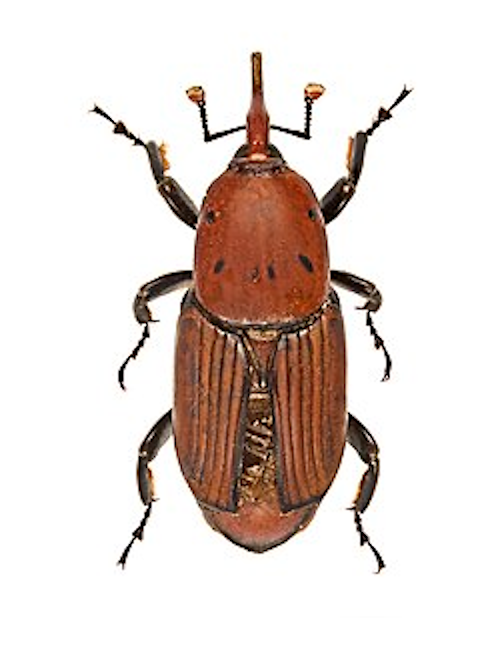
\includegraphics[scale=1]{./Figures/picudo-rojo.png}
  \caption{Picudo rojo\protect\footnotemark.}
  \label{fig:picudo-rojo}
\end{figure}

\footnotetext{Imagen tomada de \url{https://es.wikipedia.org/wiki/Rhynchophorus_ferrugineus}}

Este escarabajo supone una amenaza grave para las palmeras, ya que una vez infectada, como puede verse en la figura \ref{fig:palmera-infectada}, sus larvas se alimentan de su tejido interno, causando el colapso estructural de estos árboles en un período entre 8 y 10 meses \comment{TODO: Poner referencia}. Esta amenaza aumenta según la época del año, ya que el insecto tiene diferentes tasas de dispersión y reproducción dependiendo de la temperatura y la humedad. Existen varios tipos de picudos \comment{TODO: Poner referencia a los tipos de picudos}, algunos autóctonos y otros introducidos.

La plaga del picudo rojo llegó al Uruguay en 2022 \comment{TODO: Poner referencia}, esparciéndose rápidamente por la ciudad de Montevideo (de las 25.000 palmeras que forman una parte esencial de la ciudad, muchas ya han sucumbido a la plaga, donde se estima que para el año 2030 el ecosistema se verá ampliamente afectado \comment{TODO: Poner referencia -> Estimaciones de Alfonso}). Sin embargo, últimamente también se ha esparcido por el interior del país, como puede observarse en la figura \ref{fig:palmeras-ruta5}, perteneciente a la ruta 5 de Uruguay, donde se han encontrado palmeras muertas por la plaga.

\begin{figure}[!htpb]
  \centering
  \begin{subfigure}[b]{0.49\textwidth}
    \centering
    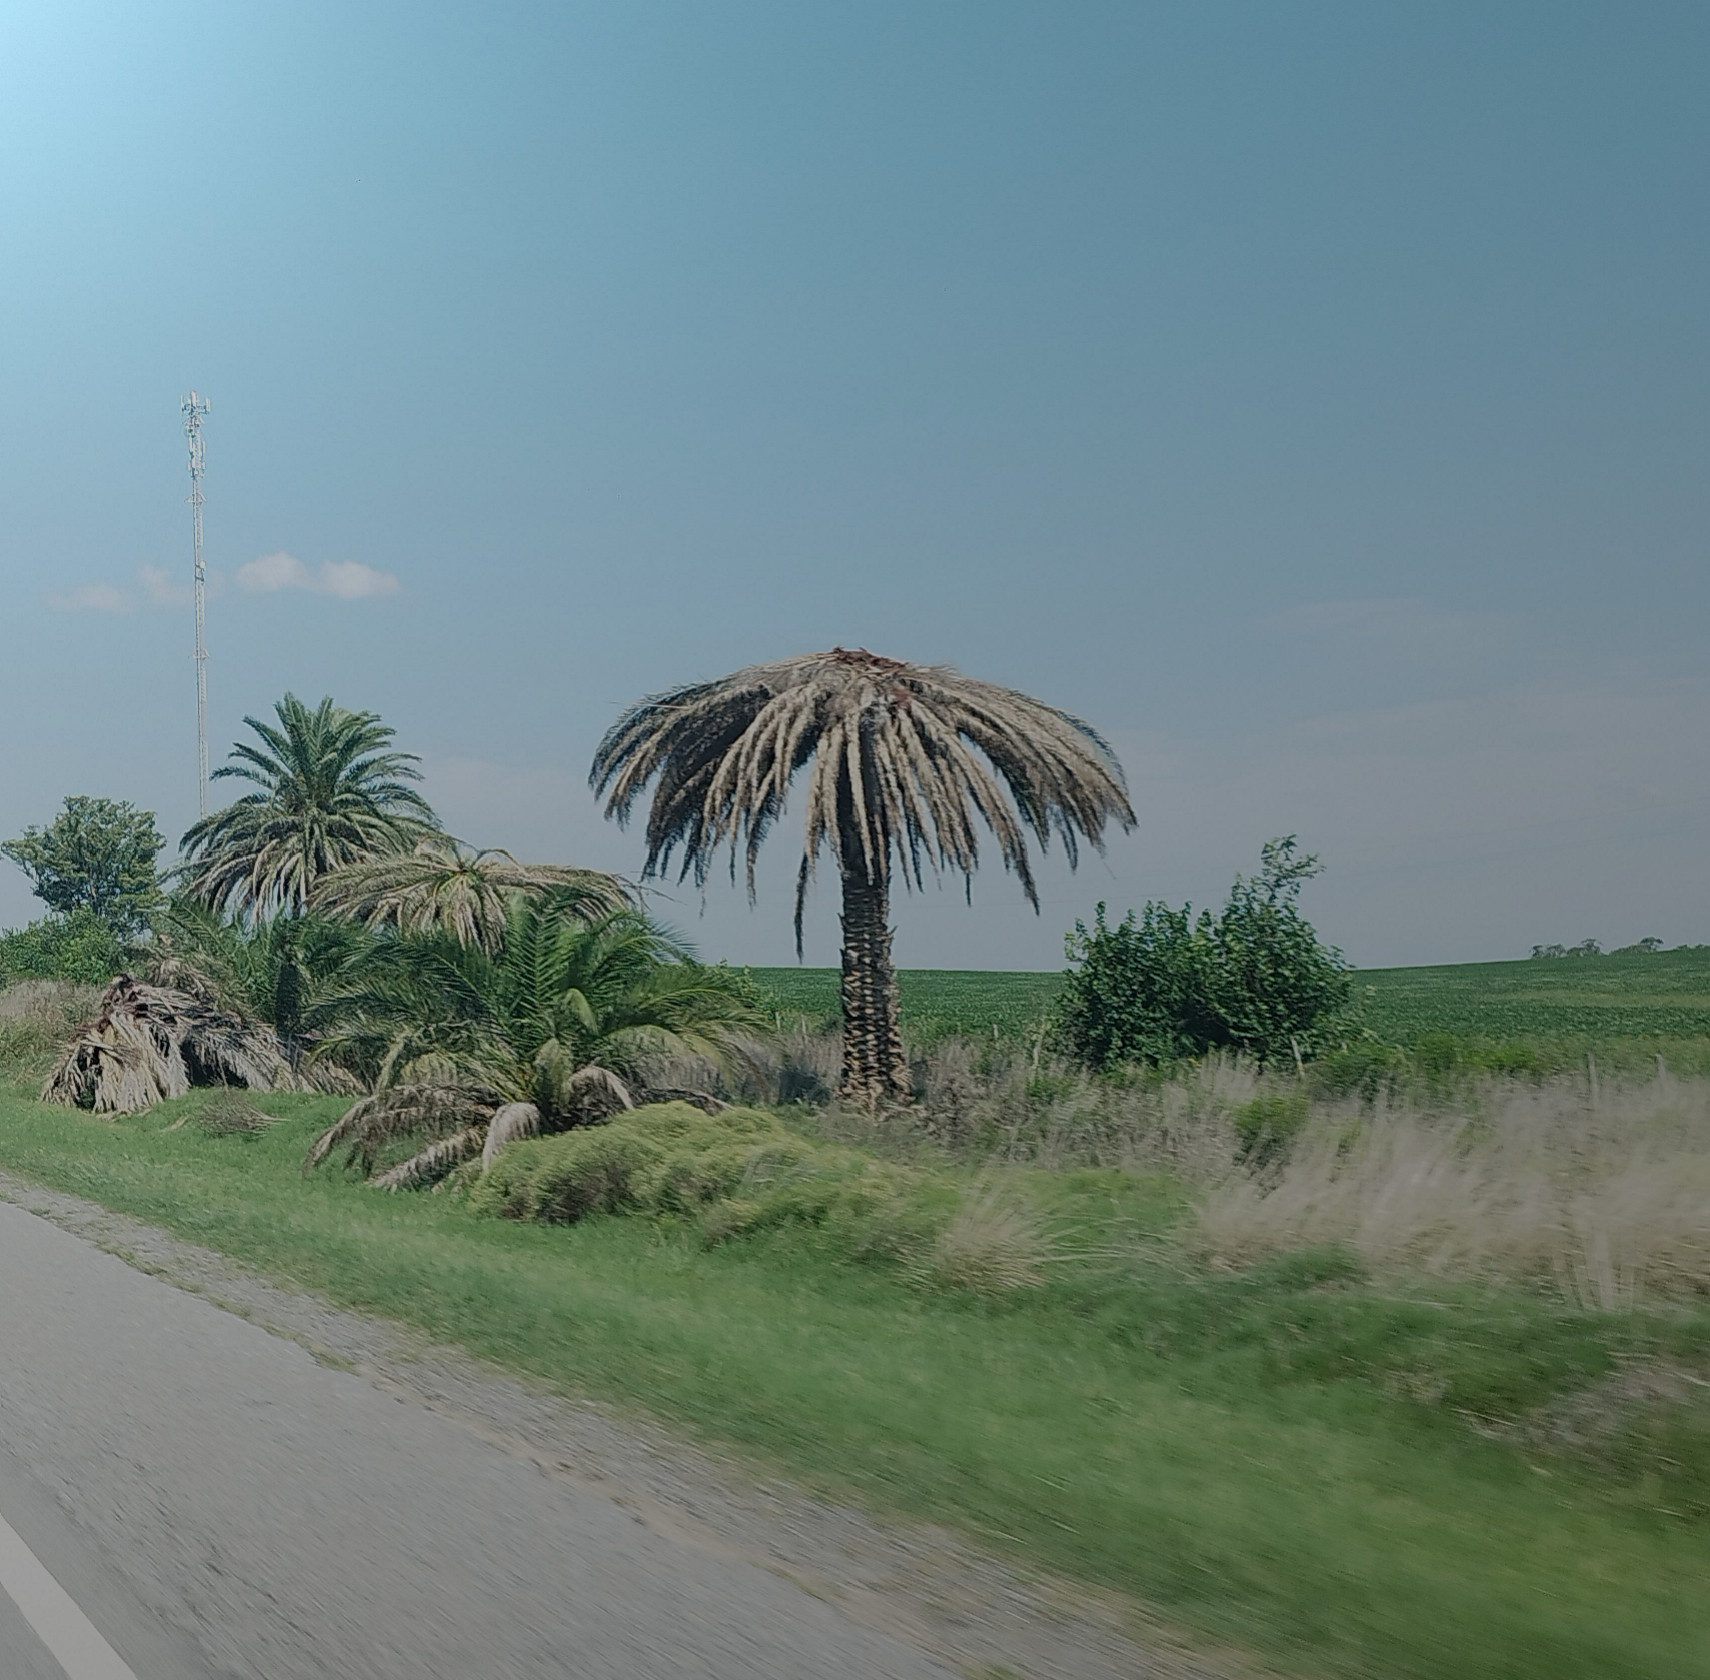
\includegraphics[width=\textwidth]{./Figures/palmera-infectada.jpg}
    \caption{Palmera infectada por el picudo rojo.}
    \label{fig:palmera-infectada}
  \end{subfigure}
  \hfill
  \begin{subfigure}[b]{0.49\textwidth}
    \centering
    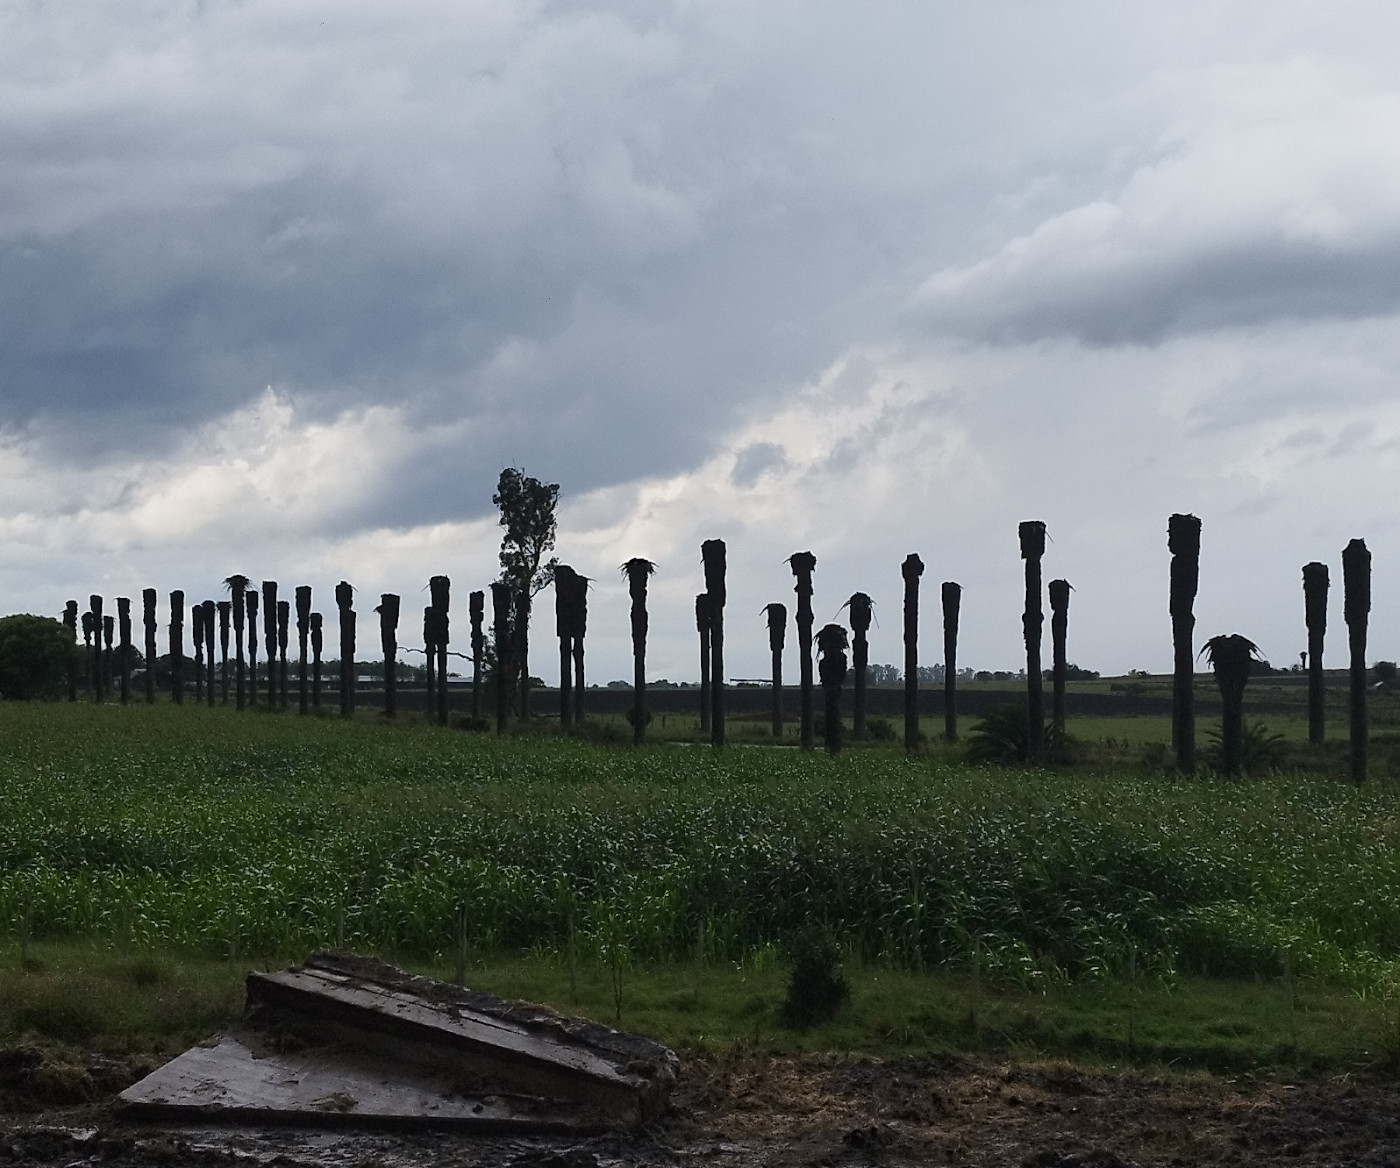
\includegraphics[width=.99\textwidth]{./Figures/palmeras-ruta5.jpg}
    \caption{Palmeras muertas en la ruta 5 de Uruguay.} 
    \label{fig:palmeras-ruta5}
  \end{subfigure}
  \caption{Infección y muerte de palmeras por el picudo rojo.}
  \label{fig:infeccion-y-muerte-palmeras}
\end{figure}

Entre los métodos de control fitosanitarios que se utilizan para combatir la plaga, se encuentran: endoterapia, baño, cirugía y remoción. \comment{TODO: Estos tratamientos se explican en el anexo 1.1}. Sin embargo, estos métodos son costosos y requieren de un monitoreo constante para detectar la presencia del picudo rojo. Para la IM no es solamente una cuestión ecológica sino también económica. En este sentido, el servicio de Arbolado realiza un seguimiento de las palmeras afectadas por la plaga. Para ello, se registra su ubicación y estado de salud, mediante campañas de detecciones a pie. Este proceso manual requiere de mucho tiempo y recursos humanos, por lo que resulta imprescindible un sistema automatizado que permita detectar la presencia de la plaga en lugares específicos de Montevideo.

Uno de los recursos aún no explotados por la IM para el monitoreo de la plaga es el uso de imágenes aéreas obtenidas mediante drones, disponibles por el servicio de Geomática de esta institución. Estos ortomosaicos, que se puede observar un ejemplo en la figura \ref{fig:ejemplo-ortomosaico}, permiten obtener información detallada sobre el estado de las palmeras y su entorno. Sin embargo, el análisis de estas imágenes es un proceso complejo que requiere de técnicas avanzadas de procesamiento de imágenes y aprendizaje automático, así como también herramientas que brinden soporte a estas actividades.

\begin{figure}[H]
  \centering
  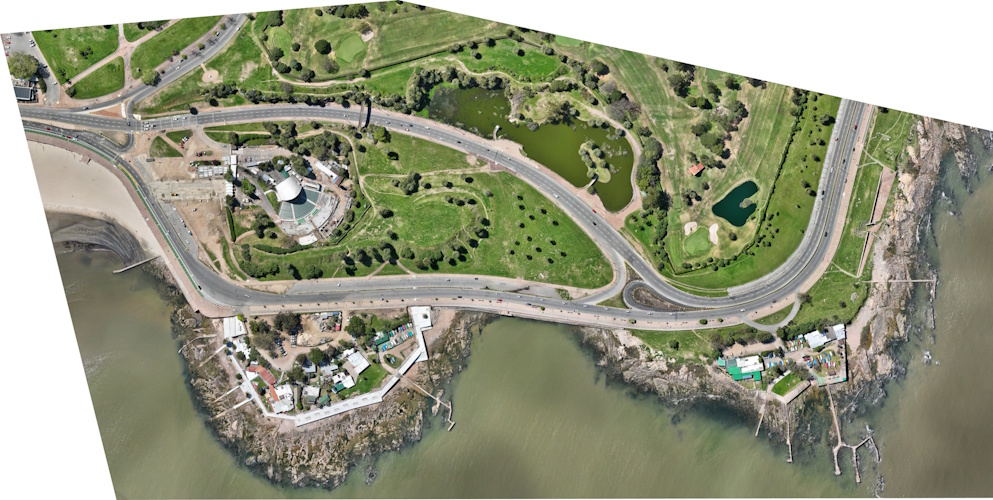
\includegraphics[scale=0.3]{./Figures/ejemplo-ortomosaico.jpg}
  \caption{Ejemplo de ortomosaico\protect\footnotemark.}
  \label{fig:ejemplo-ortomosaico}
\end{figure}

\footnotetext{Imagen tomada del sistema de información geográfica de la IM (SIG): \url{https://sig.montevideo.gub.uy/}}

% Poner ortomosaicos

%--------------------------------------------------------------------------------------------------------------------------------------------------------------------------------
\section{Estado del arte}
\label{sec:estadoArte}

% Trabajos similares sobre identificación de la plaga en otras partes del mundo.
% Incluir cuadro comparativo entre papers.

%--------------------------------------------------------------------------------------------------------------------------------------------------------------------------------

\section{Objetivos y alcance}
\label{sec:objetivos}

% Objetivos para la intendencia de Montevideo y objetivos técnicos. Alcance: anotaciones y modelado.